%=====================================================================
\section{Admission across owners without disclosure}\label{sec:protocol}

Algorithm~\ref{alg:admit} needs, for slots whose rules belong to several owners, findings that no owner can compute alone. This section computes them on secret shares so that each owner learns the findings that involve it and nothing else beyond a stated leakage. Slots of a single owner are evaluated by that owner in the clear.

\subsection{Building blocks}\label{sec:mpcbasics}
Two servers $S_1, S_2$ hold additive shares $\shr{x} = (x_1, x_2)$ with $x = x_1 + x_2$ in $\Fp$, $p = 2^{31}-1$. Additions and multiplications by public constants are local. A product $\shr{xy}$ uses a Beaver triple $(\shr{a}, \shr{b}, \shr{ab})$ from a dealer~\cite{beaver1991triples}: the servers open $d = x - a$ and $e = y - b$ and set $\shr{xy} = \shr{ab} + d\shr{b} + e\shr{a} + de$. An input matrix $X$ is masked once by a random matrix $A$ and $X - A$ is opened; products $X Y^{\top}$ of masked inputs then need no further interaction, given shares of $A_X A_Y^{\top}$ from the dealer. Outputs are sent by both servers to the owner entitled to them, never opened to the servers.

\subsection{Same-layer pairs as inner products}\label{sec:pairsecure}
Write $\chi_a(e) \in \{0,1\}^{D_a}$ for the indicator of $c(a)$, a wildcard being the full domain, and $\chi(e)$ for the concatenation over $a \in A_\ell$. For two rules, $\langle \chi_a(e), \chi_a(e')\rangle = |c(a) \cap c'(a)|$. With $x_{ee'} = \eta_e + \eta_{e'} - 2\eta_e\eta_{e'}$, where $\eta \in \{0,1\}$ encodes the effect, \Cref{lem:overlap,lem:subsume} give
\begin{align}
e \text{ conflicts with } e' &\iff x_{ee'} \textstyle\prod_{a \in A_\ell} \langle \chi_a(e), \chi_a(e')\rangle \neq 0, \label{eq:secconf}\\
e \text{ is redundant w.r.t.\ } e' &\iff \bigl(|\chi(e)| - \langle \chi(e), \chi(e')\rangle\bigr) + x_{ee'} = 0, \label{eq:secred}
\end{align}
because $|\chi(e)| - \langle \chi(e), \chi(e')\rangle = \sum_a |c(a) \setminus c'(a)|$. Every factor is an integer smaller than $|V_\ell| + 2 < p$, so a product in $\Fp$ is zero exactly when one factor is. \Cref{fig:incidence} works the tests on three rows. Algorithm~\ref{alg:pairsecure} applies these tests to the rule $e$ of an event and the foreign rules $J$ that share a key vertex with it.


\begin{figure}[t]
\centering
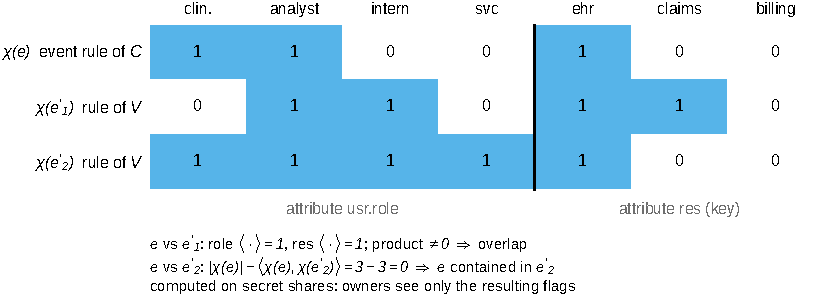
\includegraphics[width=0.85\linewidth]{figures/fig_incidence.pdf}
\caption{Incidence rows of three rules over two attributes. Per-attribute inner products give overlap, and $|\chi(e)|-\langle\chi(e),\chi(e')\rangle$ gives containment; the servers evaluate these on secret shares.}\label{fig:incidence}
\end{figure}
\begin{algorithm}[t]
\caption{$\textsc{PairSecure}(e, J)$: same-layer findings between an event's rule and foreign rules}\label{alg:pairsecure}
\begin{algorithmic}[1]
\Require rule $e$ of the event's owner; rules $J = (e'_1, \dots, e'_N)$ of other owners with $\key(e'_j) \cap \key(e) \neq \emptyset$
\Ensure to the event's owner: whether $e$ conflicts with, or is redundant w.r.t., some $e'_j$; to the owner of $e'_j$: whether $e'_j$ conflicts with $e$ or is redundant w.r.t.\ $e$
\State each owner masks and shares its rows $\chi(\cdot)$ and effects $\eta$ \Comment{one opening per input}
\State $\shr{x_j} \gets \shr{\eta_e} + \shr{\eta_j} - 2\shr{\eta_e\eta_j}$ for all $j$ \Comment{masked products, no interaction}
\State $\shr{z_j} \gets \shr{x_j}$; \textbf{for} $a \in A_\ell$ \textbf{do} $\shr{z_j} \gets \shr{z_j} \cdot \langle \shr{\chi_a(e)}, \shr{\chi_a(e'_j)}\rangle$ \Comment{$|A_\ell|$ Beaver rounds}
\State send $\sum_j \rho_j \shr{z_j}$ (random $\rho_j$) to the event's owner; send $\rho'_j \shr{z_j}$ to the owner of $e'_j$ \Comment{conflict, \eqref{eq:secconf}}
\State $\shr{w_j} \gets |\shr{\chi(e)}| - \langle \shr{\chi(e)}, \shr{\chi(e'_j)}\rangle + \shr{x_j}$ \Comment{redundancy of $e$, \eqref{eq:secred}}
\State send $\rho \prod_j \shr{w_j}$ (random $\rho \neq 0$, product by a balanced tree) to the event's owner
\State symmetrically, send $\rho''_j\bigl(|\shr{\chi(e'_j)}| - \langle \shr{\chi(e'_j)}, \shr{\chi(e)}\rangle + \shr{x_j}\bigr)$ to the owner of $e'_j$
\State each recipient reads a flag as ``value $\neq 0$'' for conflicts and ``value $= 0$'' for redundancy
\end{algorithmic}
\end{algorithm}

\subsection{Cross-layer cells: decide locally, combine securely}\label{sec:ldsc}
For a cell $(t, r)$ whose tool host $h$ differs from the owners $K_r$ of $r$, each party evaluates its \emph{own} policy in the clear and only the conjunction of \Cref{def:cross} is computed jointly. The host computes $\tau_u = [\dec_{\mathsf{tool}}(u, t) = \permit]$ for $u \in S$. Each owner $k \in K_r$ computes, for each identity $i \in S \cup \{c\}$ where $c$ is the service account of $t$ if any, $\pi_k(i) = 1$ if one of its permit rules matches $(i, r)$ and $\delta_k(i) = 1$ if one of its deny rules does. Under deny-overrides the joint decision is
\begin{equation}
D(i) = \Bigl(1 - \prod_{k \in K_r} \bigl(1 - \pi_k(i)\bigr)\Bigr) \prod_{k \in K_r} \bigl(1 - \delta_k(i)\bigr), \label{eq:jointdec}
\end{equation}
and permit-overrides is obtained by dropping the second product. When $|K_r| = 1$ the owner computes $D$ directly, for any combining function. Algorithm~\ref{alg:ldsc} then evaluates \Cref{def:cross} with one or two products per user.

\begin{algorithm}[t]
\caption{$\textsc{CellSecure}(t, r)$: decide locally, combine securely}\label{alg:ldsc}
\begin{algorithmic}[1]
\Require host $h$ of $t$ with $\tau \in \{0,1\}^{S}$; owners $K_r$ of $r$ with local bits $\pi_k, \delta_k$ on $S \cup \{c\}$
\Ensure blocked-grant and amplification flags for $(u, t, r)$, $u \in S$, to $h$ and to the owners of $r$
\State all parties share their bit vectors
\State $\shr{D} \gets$ \eqref{eq:jointdec} with $2(|K_r| - 1) + 1$ products of vectors \Comment{skipped if $|K_r| = 1$}
\If{$\beta_t = \obo$}
  \State $\shr{g_u} \gets \shr{\tau_u}(1 - \shr{D(u)})$;\quad $\shr{a_u} \gets 0$
\Else \Comment{$\beta_t = \svc(c)$}
  \State $\shr{g_u} \gets \shr{\tau_u}(1 - \shr{D(c)})$;\quad $\shr{a_u} \gets \shr{\tau_u}\shr{D(c)}(1 - \shr{D(u)})$
\EndIf
\State send $\shr{g}$ and $\shr{a}$ to the recipients (or only $\rho \sum_u \shr{g_u}$ and $\rho' \sum_u \shr{a_u}$ in \emph{existence-only} mode)
\end{algorithmic}
\end{algorithm}

Usage and drift cells need no cryptography. The owner of a resource must see the description of every tool that reads it in order to approve it; it therefore evaluates $\Viol$ and $\Drift_t$ on its own usage rules and the disclosed description, and tells the host which elements are violated.

\begin{figure}[t]
\centering
\resizebox{\linewidth}{!}{%
\begin{tikzpicture}[font=\scriptsize, >=Stealth, x=1cm, y=0.6cm,
  lbl/.style={fill=white, inner sep=1pt}]
\foreach \x/\n in {0/{Owner $V$ (event)},3.4/{Owner $C$},6.8/{Server $S_1$},10.2/{Server $S_2$},13.6/{Dealer}}{
  \node[draw, fill=gray!10, rounded corners=1pt, minimum width=2.2cm, align=center] at (\x,0) {\n};
  \draw[gray] (\x,-0.6) -- (\x,-13.0);}
\draw[->] (0,-1.5) -- node[lbl, above] {1. event $\epsilon$: opaque id and key vertices} (3.4,-1.5);
\node[draw, fill=yellow!15, align=center, font=\scriptsize] at (1.7,-3.0) {2. both owners: $\textsc{Region}(\epsilon)$ from the index;\\ evaluate their own rules on the region};
\draw[->] (0,-4.6) -- node[lbl, above, pos=0.62] {3. shares of $V$'s inputs} (6.8,-4.6);
\draw[->] (0,-4.9) -- (10.2,-4.9);
\draw[->] (3.4,-5.9) -- node[lbl, above, pos=0.35] {3. shares of $C$'s inputs} (6.8,-5.9);
\draw[->] (3.4,-6.2) -- (10.2,-6.2);
\draw[->] (13.6,-7.3) -- node[lbl, above] {4. triples} (10.2,-7.3);
\draw[->] (13.6,-7.6) -- (6.8,-7.6);
\draw[<->] (6.8,-8.8) -- node[lbl, above] {5. open $d$, $e$ (Beaver)} (10.2,-8.8);
\draw[<->] (6.8,-9.4) -- node[lbl, below] {one exchange per round} (10.2,-9.4);
\draw[->] (6.8,-10.6) -- node[lbl, above, pos=0.5] {6. output shares} (3.4,-10.6);
\draw[->] (10.2,-10.9) -- (3.4,-10.9);
\draw[->] (6.8,-11.5) -- (0,-11.5);
\draw[->] (10.2,-11.8) -- (0,-11.8);
\node[draw, fill=green!10, align=center, font=\scriptsize] at (1.7,-12.6) {7. each owner reconstructs its findings; accept or hold};
\end{tikzpicture}}
\caption{Message flow of one admission across two owners. Servers see only uniformly random shares and openings; each owner receives only the outputs that concern its rules, tools or resources.}\label{fig:sequence}
\end{figure}

\subsection{Security}\label{sec:security}
Let $\mathcal{F}_\epsilon$ be the functionality that receives the fragments of the owners of $\Reg(\epsilon)$ and returns to each of them the findings of the region that involve its rules, tools or resources, in the granularity of Algorithms~\ref{alg:pairsecure} and~\ref{alg:ldsc}. Let the leakage $\mathcal{L}(\epsilon)$ consist of: the key vertices of $\epsilon$ and the identifiers of the owners in its region; the number of rules each owner holds on each key vertex of the region; the population size $|S|$; the bindings of the tools in the region and, to the owner of a resource, the descriptions of the tools that read it.

\begin{theorem}[Security]\label{thm:security}
Against a semi-honest adversary that corrupts one server, or any set of owners but no server, the protocol formed by Algorithms~\ref{alg:pairsecure} and~\ref{alg:ldsc} and the local usage check computes $\mathcal{F}_\epsilon$ with leakage $\mathcal{L}(\epsilon)$: there is a simulator that, given only the corrupted parties' inputs, outputs and $\mathcal{L}(\epsilon)$, produces a view whose distribution is identical to the real view for a corrupted server and within statistical distance $q/p$ for a coalition of owners that receives $q$ conflict outputs.
\end{theorem}
\begin{proof}[Proof sketch]
We follow the simulation paradigm~\cite{goldreich2004foundations}. \emph{Corrupted server.} Its view consists of (i) one share of every input, (ii) the openings $d = x - a$, $e = y - b$ and $X - A$, and (iii) its own randomness. Shares are uniform in $\Fp$ and independent of the inputs. Each opening is the input minus a value $a$, $b$ or $A$ that is uniform and unknown to the server, since the dealer shares it and the other server does not collude; openings for distinct products use fresh triples, and a masked input is opened once and then reused only in local products. The view is therefore a vector of independent uniform elements whose length is fixed by the number of rules per key vertex, $|S|$, $|A_\ell|$ and the bindings, all of which are in $\mathcal{L}(\epsilon)$. The simulator samples such a vector. Outputs are not sent to servers.
\emph{Corrupted owners.} Their view consists of their own inputs, shares they produce, and the values sent to them. Blocked-grant and amplification bits, and the local usage results, are outputs of $\mathcal{F}_\epsilon$. A redundancy value $\rho \prod_j w_j$ with $\rho$ uniform in $\Fp^{*}$ is $0$ when the flag is set and uniform in $\Fp^{*}$ otherwise, which the simulator reproduces from the flag. A conflict value $\sum_j \rho_j z_j$ with $\rho_j$ uniform in $\Fp$ is $0$ when no $z_j \neq 0$ and uniform in $\Fp$ otherwise; the simulator outputs $0$ or a uniform element, which differs from the real distribution only by the event that a uniform element equals $0$, of probability $1/p$ per output.
\end{proof}

\begin{proposition}[Correctness]\label{prop:correct}
Algorithms~\ref{alg:pairsecure} and~\ref{alg:ldsc} return the findings of \Cref{def:pair,def:cross} exactly, except that a conflict existence flag is missed with probability at most $1/p$ per output.
\end{proposition}
\begin{proof}
By \eqref{eq:secconf}, \eqref{eq:secred} and \eqref{eq:jointdec}, each flag is a product of field elements that are integers below $p$; $\Fp$ has no zero divisors, so the product is zero exactly when a factor is. Blocked-grant and amplification bits are products of bits and are opened directly. Redundancy uses a non-zero multiplier and is exact. The conflict existence value $\sum_j \rho_j z_j$ is zero for some non-zero $(z_j)$ with probability $1/p$ over the $\rho_j$.
\end{proof}
The prototype uses $p = 2^{31}-1$ for speed; a 61-bit prime reduces the error and the statistical distance of \Cref{thm:security} to $2^{-61}$ per output at about twice the communication.

\subsection{What the findings themselves reveal}\label{sec:outputleak}
Theorem~\ref{thm:security} bounds what the protocol reveals beyond the findings, not what the findings reveal. An owner can submit events crafted to learn another owner's decisions.

\begin{proposition}[Probing]\label{prop:probe}
(i) With per-user outputs, a tool host that submits a tool rule permitting every $u \in S$ on a tool that reads $r$ on behalf of the user learns $\dec_{\mathsf{data}}(u, r)$ for all $u \in S$ from one event. (ii) With existence-only outputs, each event reveals at most one bit per output, so learning a decision row whose $|S|$ entries are independent with $\Pr[\deny] = q$ requires at least $|S| \cdot H(q)$ events in expectation, where $H$ is the binary entropy.
\end{proposition}
\begin{proof}
(i) Under $\obo$, the blocked-grant flag of $(u, t, r)$ equals $1 - D(u)$ for every $u$ with $\tau_u = 1$. (ii) An event yields one binary output; by Shannon's source coding theorem, identifying a random row requires on average at least its entropy $|S| \cdot H(q)$ in bits.
\end{proof}
Part~(i) holds for any mechanism that tells a tool host which of its users would be refused, encrypted or not; it is the price of an actionable finding. Owners choose per resource between per-user outputs and existence-only outputs with a quota of events per period, which bounds the leakage to the quota in bits. Section~\ref{sec:leakeval} measures both modes.

\subsection{Cost}\label{sec:cost}
\begin{proposition}[Communication]\label{prop:comm}
For an event rule and $N$ foreign rules on its key vertices, Algorithm~\ref{alg:pairsecure} opens $O((N+1)|V_\ell|)$ elements, performs $O(N|A_\ell|)$ Beaver products in $|A_\ell| + \lceil \log_2 N \rceil + 2$ rounds, and sends $O(N)$ output elements. For a cell with $|K_r|$ owners, Algorithm~\ref{alg:ldsc} shares $O(|S||K_r|)$ elements and performs $O(|S||K_r|)$ products in $O(|K_r|)$ rounds.
\end{proposition}
\begin{proof}
By inspection of the algorithms; the redundancy product over $N$ factors is evaluated by a balanced tree.
\end{proof}
The servers' work is linear in the region rather than in the state, as in Proposition~\ref{prop:cost}. The dealer produces triples and matrix triples whose number is of the same order; replacing it by a two-party preprocessing protocol based on oblivious transfer or homomorphic encryption removes the trusted dealer at a cost we do not measure here.
